%!TEX root = ../main.tex
\section{Background} 
In this section, we first formally define the two table discovery tasks in a data lake, and the overall architecture to solve them.

\subsection{Problem Definition}~\label{subsec:def}


\noindent\textbf{\underline{Table Join Search.}}
Suppose that a data lake $\lake$ contains a large set of tables $\lake=\{T_1, T_2, ..., T_N\}$, where each table $T_i, i \in [1,N]$ has $n_i$ rows (tuples), $m_i$ columns (attributes) and each cell value is denoted by $c_{ij}$.  Given a query table $\qtable$, as well as a specific column $\qcolumn$ of $\qtable$, table join search is to find the target tables that can be joined with  $\qtable$ on $\qcolumn$.
%
Overall, it can be taken as measuring the relevance score between two columns, denoted by $R(\qcolumn, \tcolumn)$, where   $\tcolumn$ is a column  of a target table $\ttable$. The higher the score, the more likely the two columns can be joined (we can say that the two columns or two tables can be joined interchangebly, \ie $R(\qcolumn, \tcolumn)$  can also be represented as $R(\qcolumn, \ttable)$).
Note that different methods have different criteria to compute the score, like the number of overlaps or semantic similarity.
 The formal definition is as follows. 

\begin{definition}[Top-$K$ Table Join Search]
	Given $\lake$, a query table $\qtable$ and the specific column $\qcolumn$, Top-$K$ table join search aims to retrieve a subset $\lake_q \subset \lake$, $|\lake_q|=K$ such that $\forall T \in \lake_q$ and $\forall T' \in T \setminus \lake_q$, $R(\qcolumn, T)>R(\qcolumn, T')$.
\end{definition}

\noindent \underline{\textit{Remark.}} Given a target table $T_t$, there may exist multiple columns that can be joined with $\qtable$. In this way,  we  take the one with the highest score as the target column, \ie $\tcolumn=\arg\max\limits_{C\in T_t} R(\qcolumn, C)$. Also, we just focus on the single join rather than multiple joins like~\cite{}.

\noindent\textbf{\underline{Table Union Search.}} Given a query table $\qtable$,  table union search aims at finding the most top-$K$ unionable tables from the data lake $\lake$. At a high level, the foundation of table union search is still the unionbility of  columns, \ie a pair of unionable tables should have multiple pairs of columns to be unioned. Similar to the table join search, the column unionbility also considers the overlaps and/or semantics between columns. To be specific, given a target table $\ttable$, we can compute the relevance of each pair of columns, \ie   $R(C, C), C \in \qtable, C' \in \ttable$, and then a table-level relevance score can be computed as $R(\qtable, \ttable)$.


\begin{definition}[Top-$K$ Table Union Search]
	Given $\lake$ and a query table $\qtable$, Top-$K$ table union search aims to retrieve a subset $\lake_q \subset \lake$, $|\lake_q|=K$ such that $\forall T \in \lake_q$ and $\forall T' \in T \setminus \lake_q$, $R(\qtable, T)>R(\qtable, T')$.
\end{definition}


\noindent \underline{\textit{Remark.}} One may consider that why we return the top-$K$ results rather than just  a set of  tables that a table discovery algorithm think as the joinable/unionable results.
The reason is that in this way, we have to set a cut-off threshold for the relevance score, which is rather hard to generalize to different table discovery algorithms. Therefore, almost all~\cite{} existing works focus on retrieving the top-$K$ results.  In this case, another natural problem is that how to set an appropriate $K$. In real applications, 

\subsection{Overall Framework of Table Discovery}

In this subsection, we will introduce the high-level framework of table discovery, which generally consists of the following modules, namely column modeling, index construction, online table query processing.
At a high level, the former two modules are offline, \ie respectively representing each column in the data lake to a vector and indexing theses columns. Then, when a query table comes, the column(s) of the table is (are) first encoded. Afterwards, with the help of the offline built index, top-$K$ tables with high relevance score are retrieved from the data lake. Next, we respectively illustrate each module as shown in Figure~\ref{fig:framework}.



\noindent\textbf{Column Modeling.}
%倒排索引这里不太好办, 要改一下,现在这样肯定早晚要改
%应该先写embeddings, 再单独解释倒排那种别的,id 或者 就是cell value
%但是minhash又是属于哪一种?
As discussed in Section~\ref{subsec:def},  column representation plays a significant role in join/union search. Therefore,  initially,  columns of  original tables in $\lake$ are always represented as fixed-length vectors, shown as the colorful circles in Figure~\ref{fig:framework}.
Mostly,  these vectors can be hash codes~\cite{} (\eg generated by the minhash function) or embeddings~\cite{} (\eg generated by pre-trained language model), which are capable of supporting efficient retrieval of columns with high overlapping and/or similar semantics. Besides, there exist solutions~\cite{} that just leverage original cell values of each column to search highly overlapping columns rather than using vectors. 

%embedding vectors or hash encodings, which enables the measurement of semantics within the embedding space.
 %This is particularly valuable when dealing with highly sparse target data and ensures that subsequent procedures remain independent of data object size, ultimately contributing to the attainment of optimal efficiency. A direct idea for column modeling is to use PLM to capture semantics, related methods include \starmie and \deepjoin or utilizing some hash approaches like \dlll etc.

\noindent\textbf{Index Construction.} Building upon the  column representations, different types of approximate nearest neighbor (ANN) search indexes should be utilized to manage large table repositories seamlessly. Typically, if each column is represented as a fixed-length embedding, local sensitive hashing (LSH) or graph-based index (HNSW) can be utilized to index all the embeddings, so as to enhance the search performance.
 As an option, inverted index~\cite{} can also be employed  to  accelerate the process of finding highly overlapping columns, where each cell value is mapped with the columns that contain the value. In this case, these colorful circles can be regarded as  Column IDs rather than vectors.




%For instance, both \starmie and \deepjoin leverage the Hierarchical Navigable Small World (HNSW) approach, recognized as one of the most prominent methods in ANN. In contrast, \dlll and \tus employ Locality-Sensitive Hashing (LSH) indexes to enhance search performance. Additionally, inverted indexing is employed in \josie and \santos to effectively handle millions of search scenarios.


\noindent\textbf{Online Query Processing.}


\noindent\textbf{Relevance Score Computation.}


\begin{figure}[h]
	\centering
	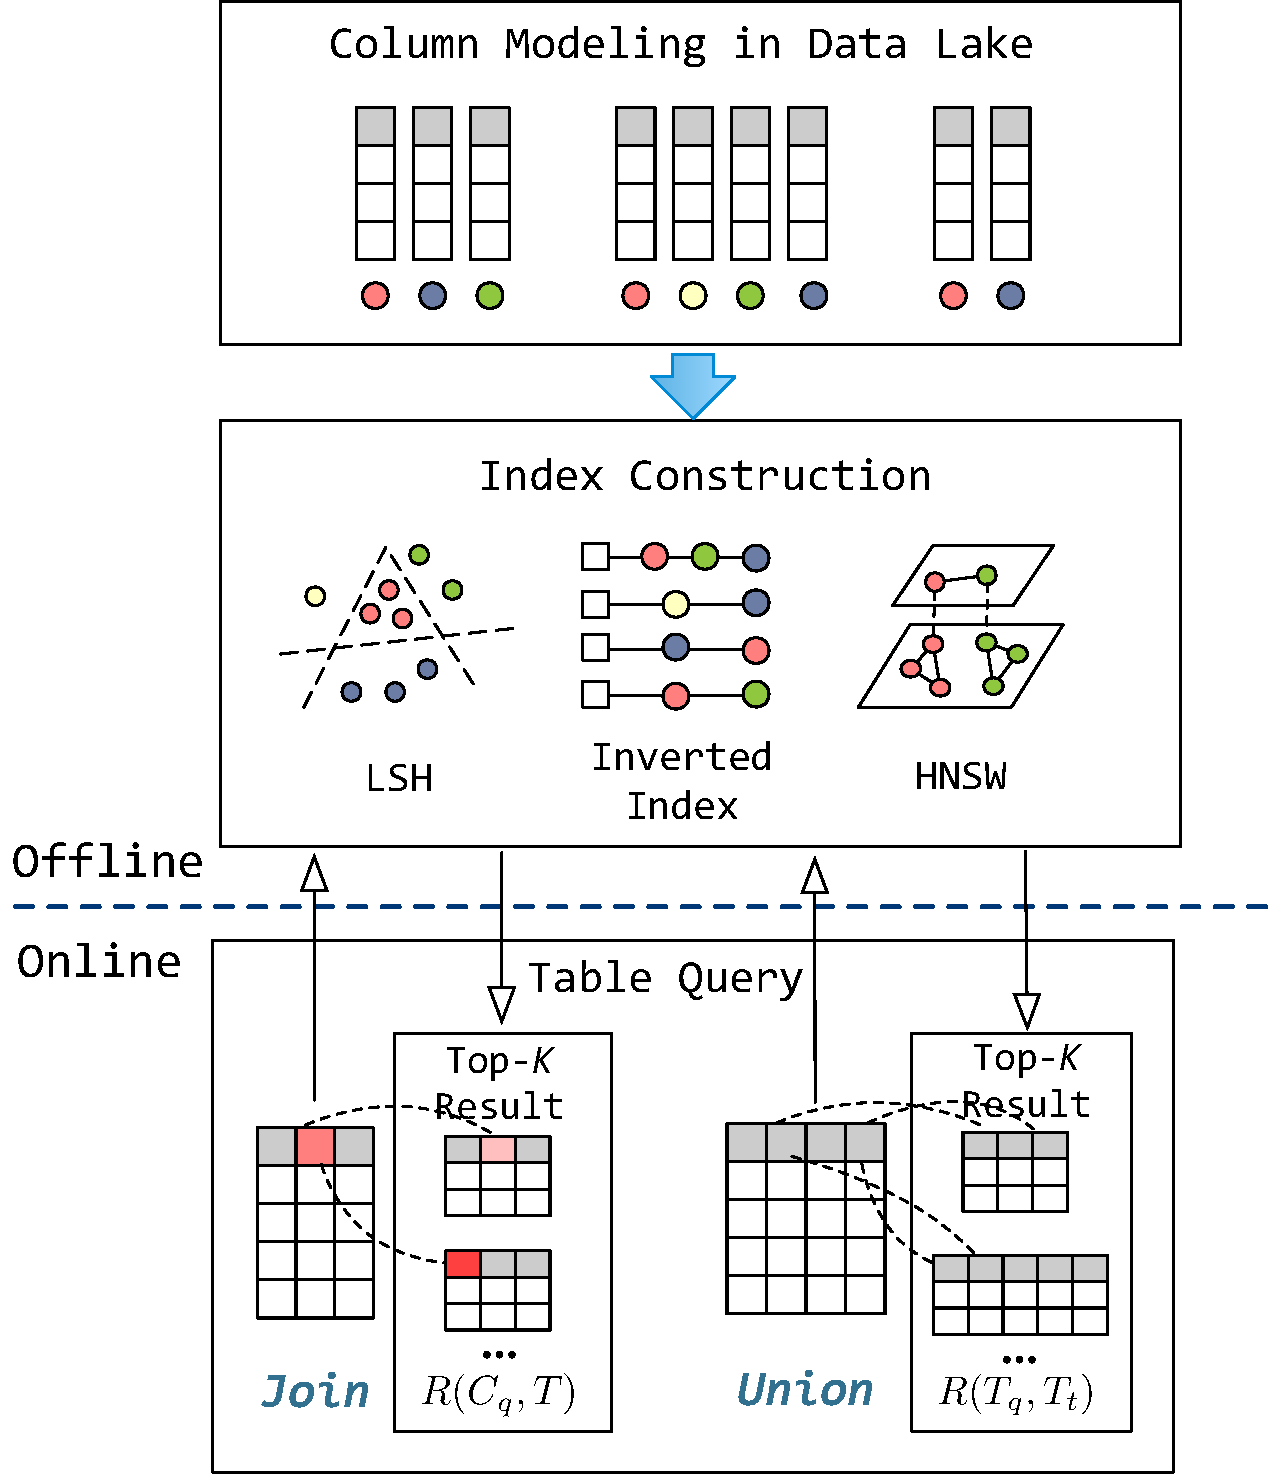
\includegraphics[width=0.95\linewidth]{fig/framework.pdf}
	\caption{Table Discovery in Data Lake.}
	\label{fig:framework}
\end{figure}




%Building upon the column encoders, we leverage cosine similarity between column embeddings to establish the column union ability score. Subsequently, we devise a bipartite matching-based method for calculating the table union ability score. Our approach introduces a filter-and-verification framework, allowing the application of diverse indexing and pruning techniques to minimize the computational load of the resource-intensive bipartite matching.

\iffalse
\subsection{Existing Benchmarks}

{\scriptsize
    
}

Arxiv work~\cite{LakeBench}
Join: 
InfoGather~\cite{InfoGather}, 
Frt12~\cite{Frt12}, 
Lsh Ensemble~\cite{LshEn}, 
Aurum~\cite{Aurum, SemProp}, 
Pexeso~\cite{Pexeso}, 
Josie~\cite{Josie}, 
DeepJoin~\cite{DeepJoin}, 




%ML Join: Metam~\cite{Metam}, Leva~\cite{Leva}, Arda~\cite{Arda}, AutoFeature~\cite{AutoFeature}


Union: 
InfoGather~\cite{InfoGather}, 
Frt12~\cite{Frt12}, 
D3L~\cite{D3L},
TUS~\cite{TUS}, 
Aurum~\cite{Aurum, SemProp}, 
Santos~\cite{Santos}
\fi



%ML Union: Starmie~\cite{Starmie}, AutoData~\cite{AutoData}